%! TeX program = lualatex
\documentclass[aspectratio=169]{beamer}
\usepackage{tikz}
\usepackage{graphicx}
\usepackage{pgfplotstable}
\usepackage{amsmath}
\usepackage{bm}
\usepackage{tcolorbox}
\tcbuselibrary{skins}
\usepackage{empheq}
\usepackage{contour}
\contourlength{1pt}
\usepackage{fontspec} 
\usepackage{xcolor}
\setsansfont{EB Garamond}
\beamertemplatenavigationsymbolsempty

\pgfplotsset{compat=1.18}
\definecolor{custombg}{HTML}{9cb6d1}
\definecolor{customeqbg}{HTML}{70a9e5}
\setbeamercolor{background canvas}{bg=custombg}

\newtcbox{\mymath}[1][]{%
    nobeforeafter,
    tcbox raise base,
    enhanced,
    colframe=black,
    colback=customeqbg,
    boxrule=1pt,
    drop shadow={
        xshift=3pt, % Removed 'shadow' prefix
        yshift=-3pt, % Removed 'shadow' prefix
        opacity=1
    },
    #1
}

\begin{document}

\begin{frame}
    \begin{tikzpicture}[remember picture,overlay]
        \node [anchor=south east] at (current page.south east) {%
            
\includegraphics[scale=0.2]{images/lab_elements.png}
        };
    \end{tikzpicture}
    \begin{tikzpicture}[remember picture,overlay]
        \node [anchor=center] at (current page.center) {%
            \begin{minipage}{\textwidth}
                \centering
                \color{black}\Huge\textbf{Étude de Lentilles minces} \\
                \color{black}\Large\textbf{L. Arsenescu et C. Bozan} \\
                \vspace{1cm}
            \end{minipage}
        };
    \end{tikzpicture}
    \begin{tikzpicture}[remember picture,overlay]
        \node [anchor=south west] at (current page.south west) {%
            
\includegraphics[scale=0.7]{images/logo_hearc_big.eps}
        };
    \end{tikzpicture}
\end{frame}

\begin{frame}
    \begin{tikzpicture}[remember picture,overlay]
        \node [anchor=south east] at (current page.south east) {%
            
\includegraphics[scale=0.2]{images/lab_elements.png}
        };
    \end{tikzpicture}
    \begin{tikzpicture}[remember picture,overlay]
        \node [anchor=north west] at ([xshift=1.4cm,yshift=-1cm]current page.north west) {%
            \color{black}\Huge\textbf{Table des matières}
        };
    \end{tikzpicture}
    \begin{tikzpicture}[remember picture,overlay]
        \node [anchor=west] at ([xshift=1.4cm]current page.west) {%
            \begin{minipage}{0.55\textwidth}
                \begin{itemize}
                    \item Buts de l'étude
                    \item Lois utilisées
                    \item Schéma de l'expérience
                    \item Déroulement de l'expérience
                    \item Comment atteindre les buts
                    \item Mesures et résultats
                    \item Conclusion
                \end{itemize}
            \end{minipage}
        };
    \end{tikzpicture}
    \begin{tikzpicture}[remember picture,overlay]
        \node [anchor=south west] at (current page.south west) {%
            \tiny \color{black}\textbf{@HE-Arc, Laboratoire de physique}
        };
    \end{tikzpicture}
\end{frame}

\begin{frame}
    \begin{tikzpicture}[remember picture,overlay]
        \node [anchor=south east] at (current page.south east) {%
            
\includegraphics[scale=0.2]{images/lab_elements.png}
        };
    \end{tikzpicture}
    \begin{tikzpicture}[remember picture,overlay]
        \node [anchor=north west] at ([xshift=1.4cm,yshift=-1cm]current page.north west) {%
            \color{black}\Huge\textbf{Buts de l'étude}
        };
    \end{tikzpicture}
    \begin{tikzpicture}[remember picture,overlay]
        \node [anchor=west] at ([xshift=1.4cm]current page.west) {%
            \begin{minipage}{0.55\textwidth}
                \begin{itemize}
                    \item Comprendre le fonctionnement des lentilles minces
                    \item Vérifier et visualiser la loi du grandissement
                \end{itemize}
            \end{minipage}
        };
    \end{tikzpicture}
    \begin{tikzpicture}[remember picture,overlay]
        \node [anchor=south west] at (current page.south west) {%
            \tiny \color{black}\textbf{@HE-Arc, Laboratoire de physique}
        };
    \end{tikzpicture}
\end{frame}

\begin{frame}
    \begin{tikzpicture}[remember picture,overlay]
        \node [anchor=north west] at ([xshift=1.4cm,yshift=-1cm]current page.north west) {%
            \begin{minipage}{0.5\textwidth}
                \Huge\textbf{Lois :} \\
                \Large\textbf{Équation de lentilles minces}
            \end{minipage}
        };
    \end{tikzpicture}
    \begin{tikzpicture}[remember picture,overlay]
        \node [anchor=south west] at ([xshift=1.4cm,yshift=1cm]current page.south west) {%
            \begin{minipage}{0.3\textwidth}
                \Large 
                \noindent \begin{empheq}[box={\mymath}]{equation*}
                    \frac{1}{f} = \frac{1}{p} + \frac{1}{q}
                \end{empheq}
                \normalsize
                \begin{itemize}
                    \item $f$ - distance focale
                    \item $p$ - distance objet
                    \item $q$ - distance image
                \end{itemize}
            \end{minipage}
        };
    \end{tikzpicture}
    \begin{tikzpicture}[remember picture,overlay]
        \node [anchor=south west] at (current page.south west) {%
            \tiny \color{black}\textbf{@HE-Arc, Laboratoire de physique}
        };
    \end{tikzpicture}
    \begin{tikzpicture}[remember picture,overlay]
        \node [anchor=south east] at ([xshift=-0.5cm, yshift=1cm]current page.south east) {%
            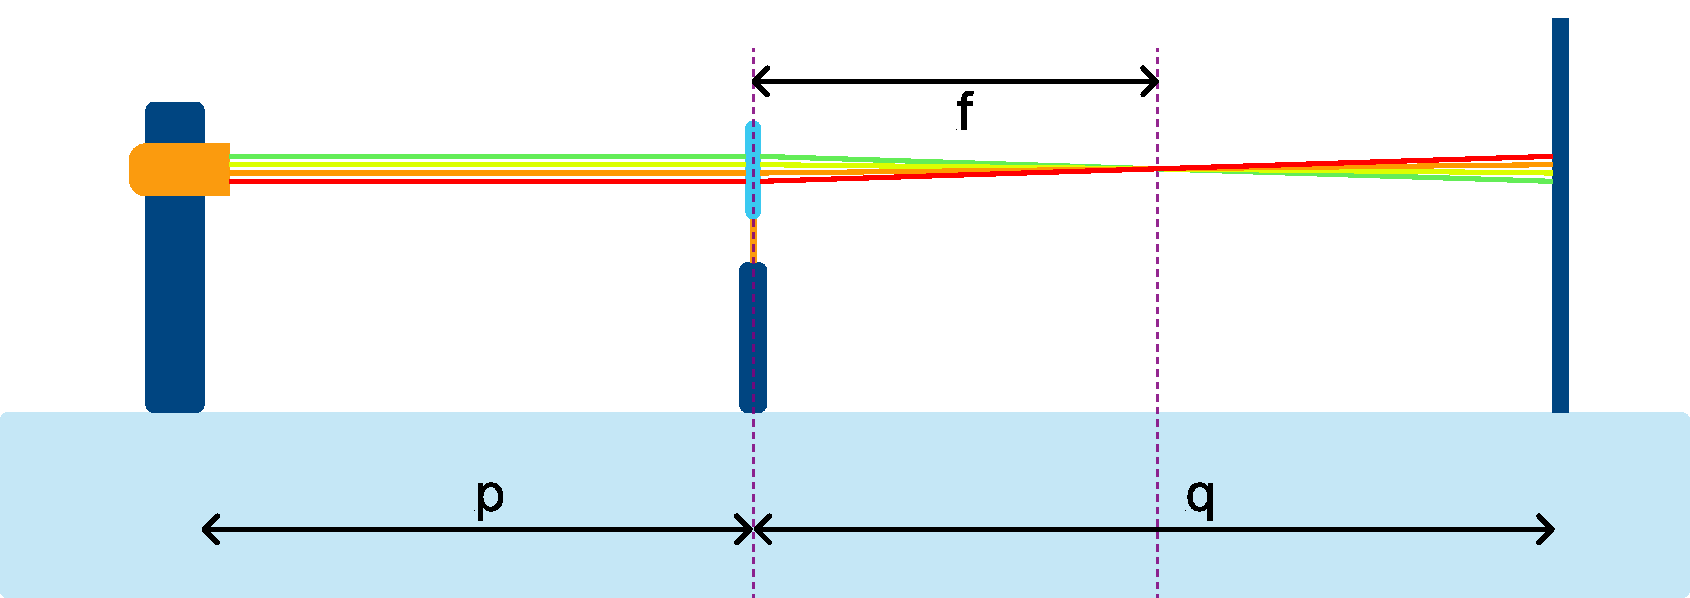
\includegraphics[width=0.55\pagewidth]{images/formule_f.pdf}
        };
    \end{tikzpicture}
    \begin{tikzpicture}[remember picture,overlay]
        \node [anchor=south west] at (current page.south west) {%
            \tiny \color{black}\textbf{@HE-Arc, Laboratoire de physique}
        };
    \end{tikzpicture}
\end{frame}


\begin{frame}
    \begin{tikzpicture}[remember picture,overlay]
        \node [anchor=north west] at ([xshift=1.4cm,yshift=-1cm]current page.north west) {%
            \begin{minipage}{0.5\textwidth}
                \Huge\textbf{Lois :} \\
                \Large\textbf{Loi du grandissement}
            \end{minipage}
        };
    \end{tikzpicture}
    \begin{tikzpicture}[remember picture,overlay]
        \node [anchor=south west] at ([xshift=1.4cm,yshift=1cm]current page.south west) {%
            \begin{minipage}{0.3\textwidth}
                \Large
                \begin{empheq}[box={\mymath}]{equation*}
                    m = \frac{y_I}{y_O} = -\frac{q}{p}
                \end{empheq}
                \normalsize
                \begin{itemize}
                    \item $m$ - grandissement
                    \item $y_I$ - hauteur image
                    \item $y_O$ - hauteur objet
                \end{itemize}
            \end{minipage}
        };
    \end{tikzpicture}
    \begin{tikzpicture}[remember picture,overlay]
        \node [anchor=south east] at ([xshift=-0.5cm, yshift=1cm]current page.south east) {%
            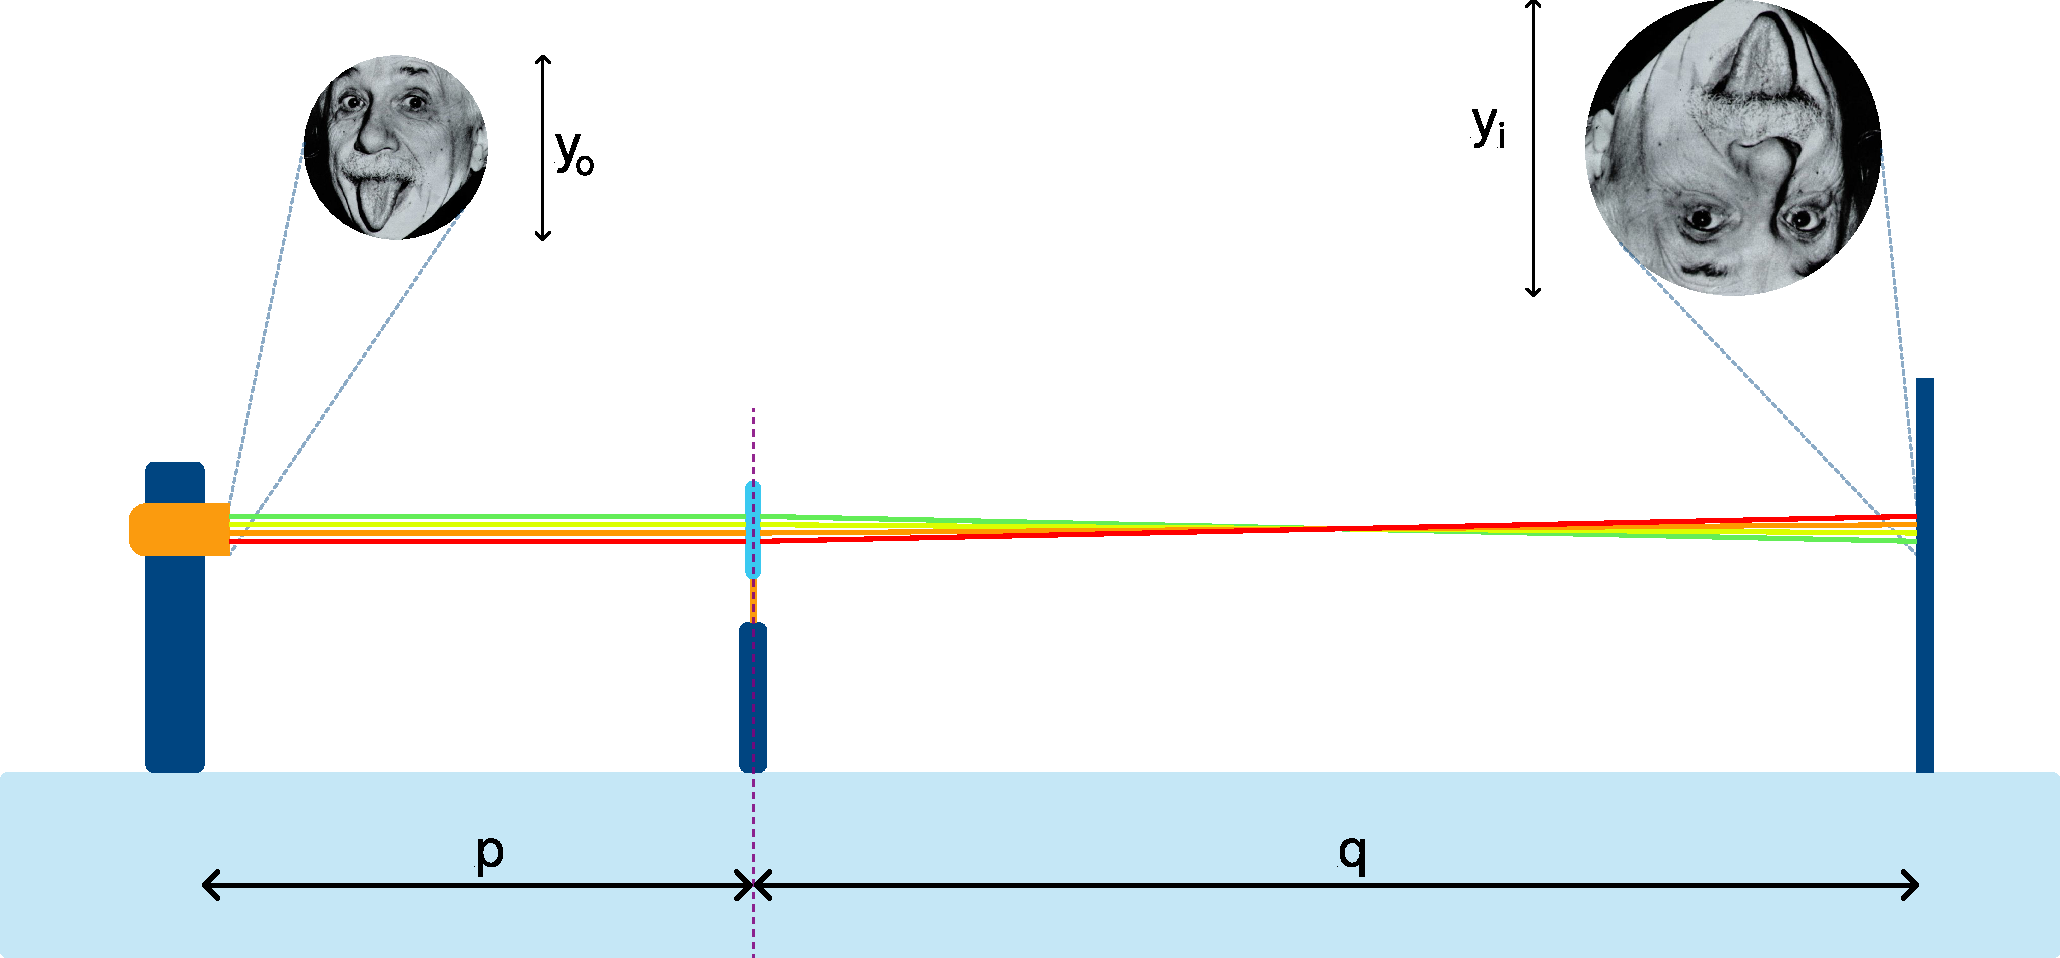
\includegraphics[width=0.55\pagewidth]{images/formule_m.pdf}
        };
    \end{tikzpicture}
    \begin{tikzpicture}[remember picture,overlay]
        \node [anchor=south west] at (current page.south west) {%
            \tiny \color{black}\textbf{@HE-Arc, Laboratoire de physique}
        };
    \end{tikzpicture}
\end{frame}

\begin{frame}
    \begin{tikzpicture}[remember picture,overlay]
        \node [anchor=north west] at ([xshift=1.4cm,yshift=-1cm]current page.north west) {%
            \color{black}\Huge\textbf{Déroulement de l'expérience}
        };
    \end{tikzpicture}
    \begin{tikzpicture}[remember picture,overlay]
        \node [anchor=south] at (current page.south) {%
            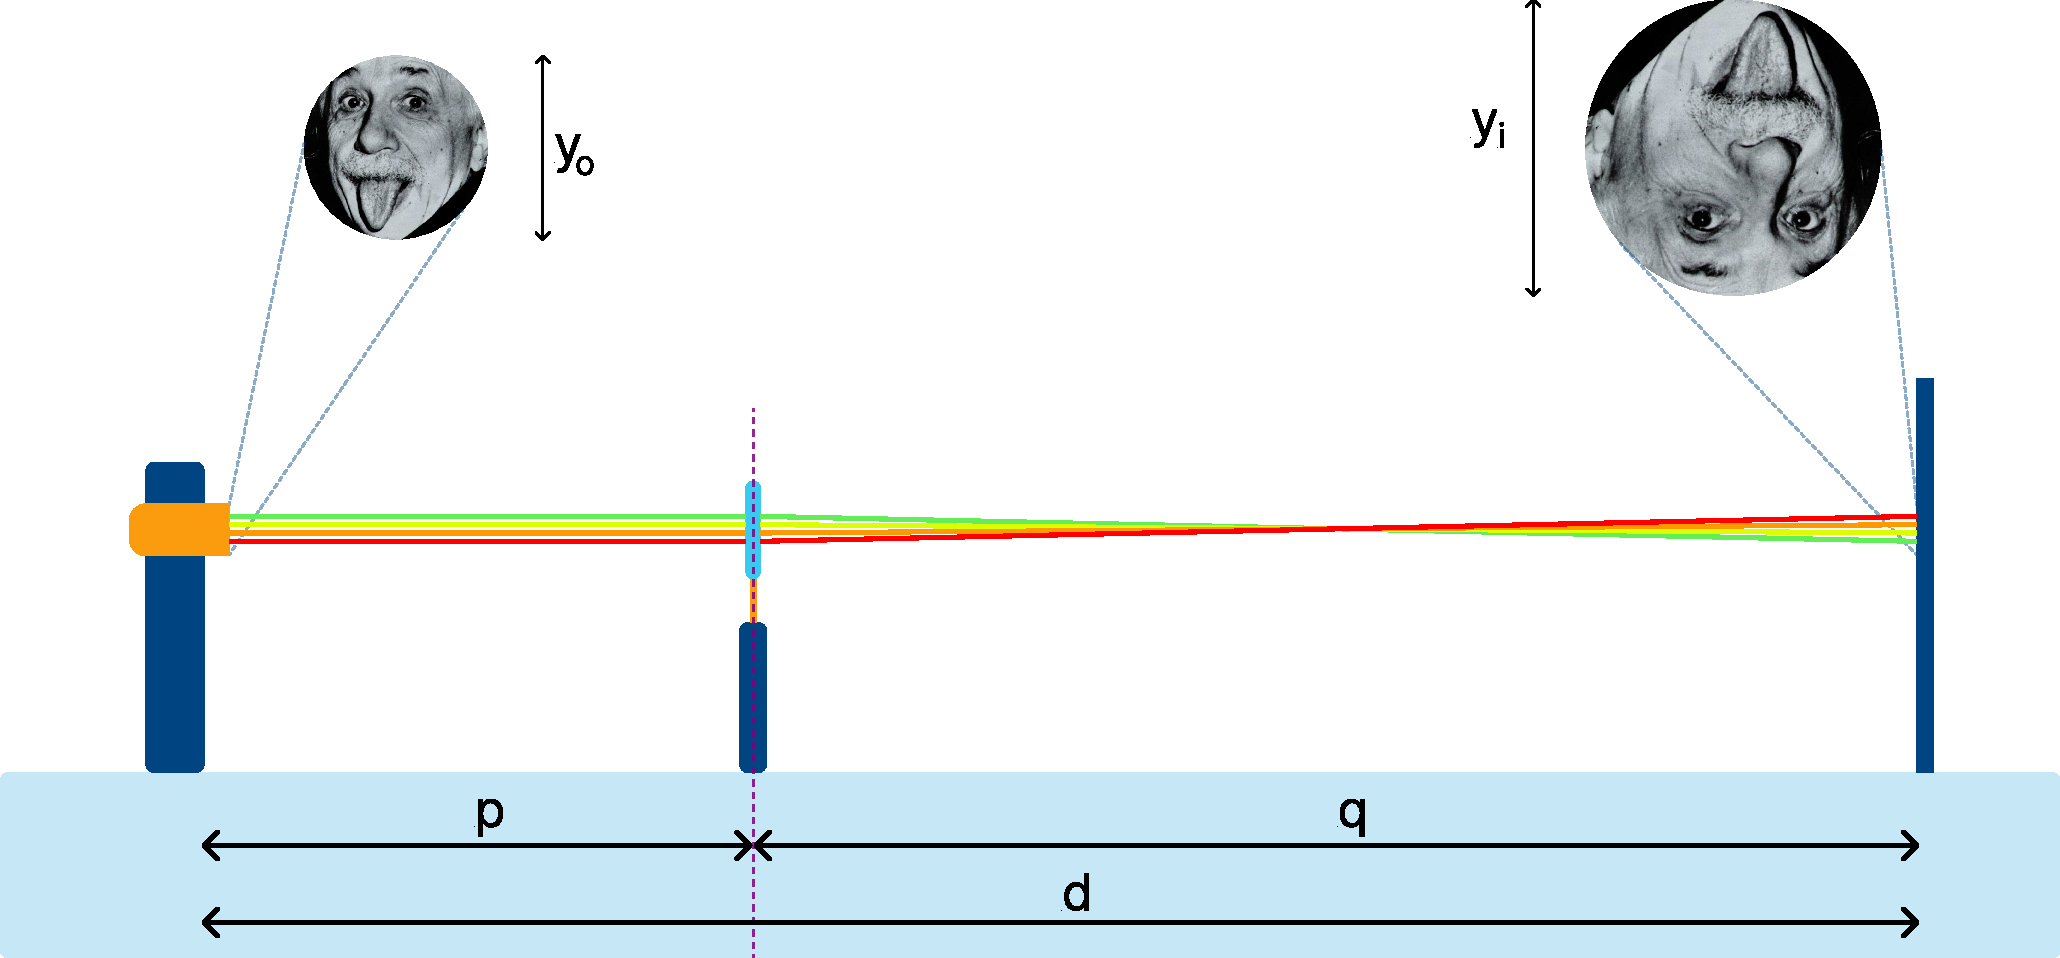
\includegraphics[width=0.8\pagewidth]{images/schema_exp.pdf}
        };
    \end{tikzpicture}
\end{frame}

\begin{frame}
    \begin{tikzpicture}[remember picture,overlay]
        \node [anchor=north west] at ([xshift=1.4cm,yshift=-1cm]current page.north west) {%
            \color{black}\Huge\textbf{Déroulement de l'expérience}
        };
    \end{tikzpicture}
    \begin{tikzpicture}[remember picture,overlay]
        \node [anchor=south west] at ([xshift=1cm, yshift=1cm]current page.south west) {%
            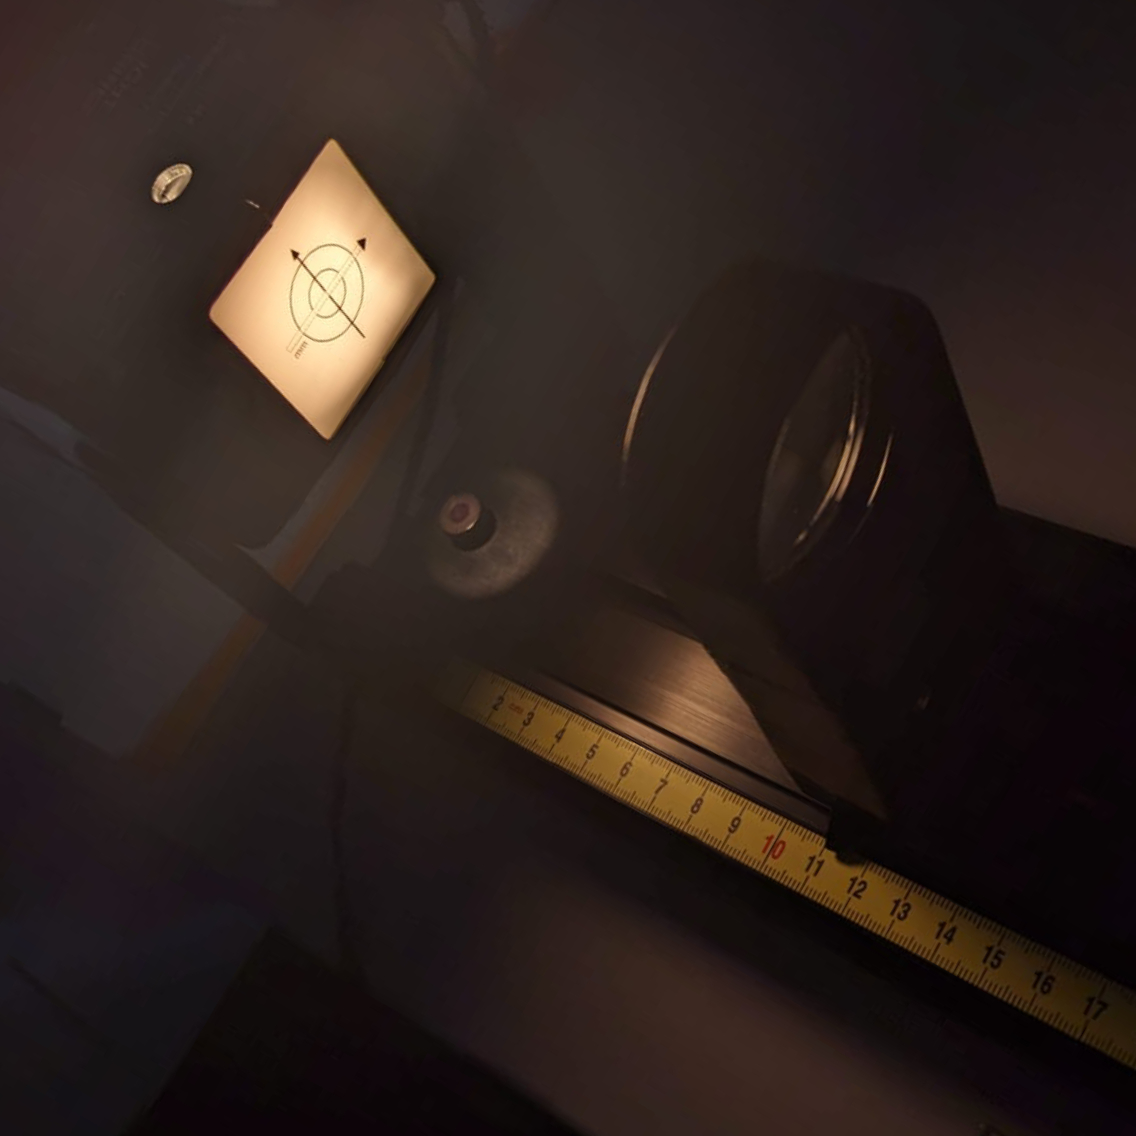
\includegraphics[width=0.35\pagewidth]{images/projector.jpg}
        };
    \end{tikzpicture}
    \begin{tikzpicture}[remember picture,overlay]
        \node [anchor=south east] at ([xshift=-1cm, yshift=1cm]current page.south east) {%
            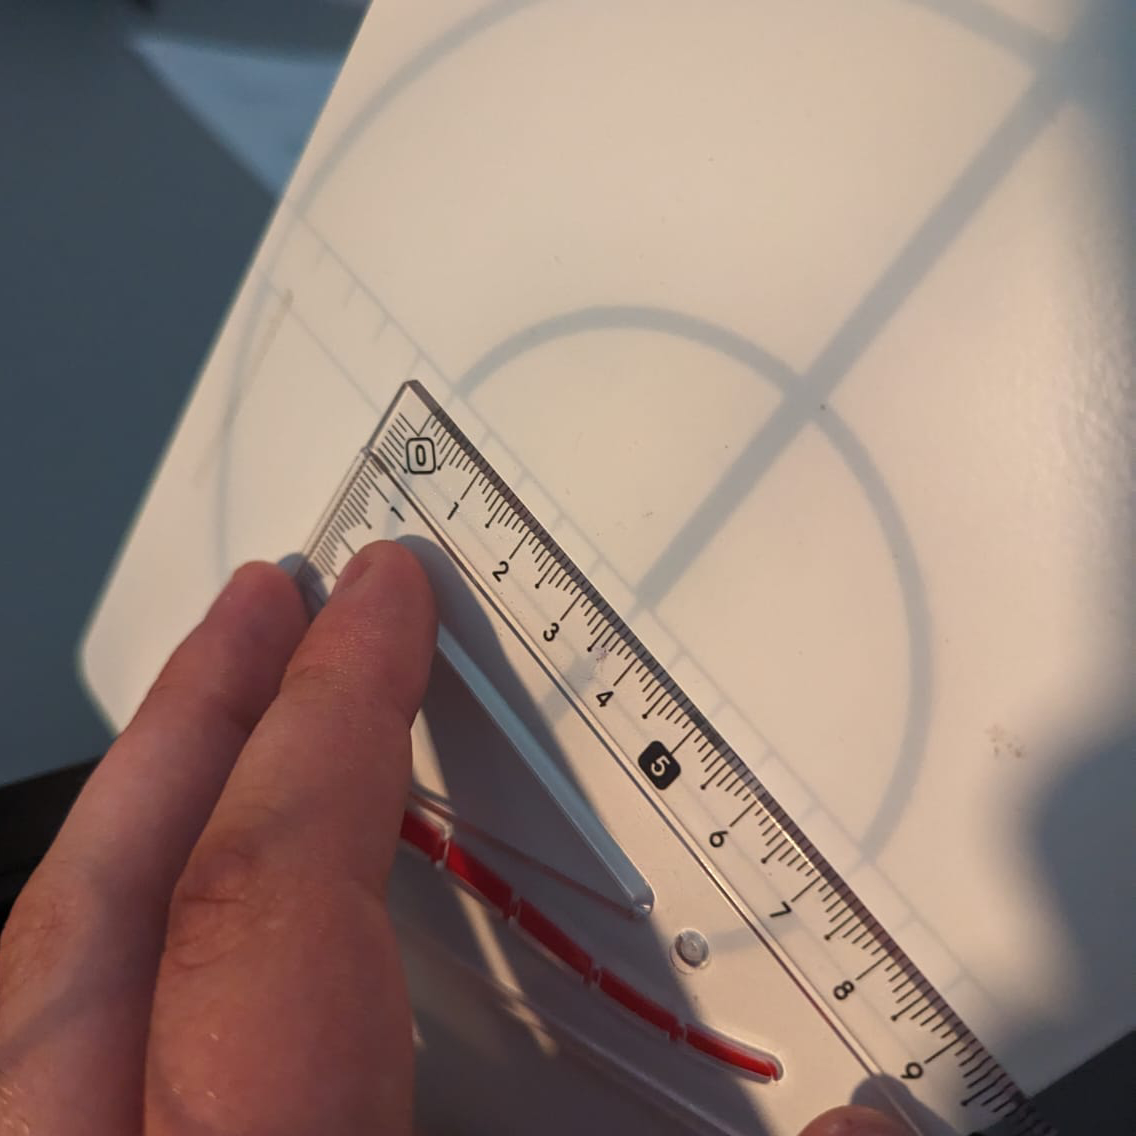
\includegraphics[width=0.35\pagewidth]{images/measuring.jpg}
        };
    \end{tikzpicture}
\end{frame}

\begin{frame}
    \begin{tikzpicture}[remember picture,overlay]
        \node [anchor=south east] at (current page.south east) {%
            
\includegraphics[scale=0.2]{images/lab_elements.png}
        };
    \end{tikzpicture}
    \begin{tikzpicture}[remember picture,overlay]
        \node [anchor=north west] at ([xshift=1.4cm,yshift=-1cm]current page.north west) {%
            \color{black}\Huge\textbf{Comment atteindre les buts}
        };
    \end{tikzpicture}
    \begin{tikzpicture}[remember picture,overlay]
        \node [anchor=west] at ([xshift=1.4cm]current page.west) {%
            \begin{minipage}{0.55\textwidth}
                \begin{itemize}
                    \item Couples de \textbf{(p, q)} pour différentes \textbf{d}
                    \item Une mesure \textbf{(p, q)} -> loi du grandissement
                    \item Les mesures \textbf{(y$\bm{_O}$, y$\bm{_I}$)} -> loi du grandissement
                \end{itemize}
            \end{minipage}
        };
    \end{tikzpicture}
    \begin{tikzpicture}[remember picture,overlay]
        \node [anchor=south west] at (current page.south west) {%
            \tiny \color{black}\textbf{@HE-Arc, Laboratoire de physique}
        };
    \end{tikzpicture}
\end{frame}

\begin{frame}
    \begin{tikzpicture}[remember picture,overlay]
        \node [anchor=south east] at (current page.south east) {%
            
\includegraphics[scale=0.2]{images/lab_elements.png}
        };
    \end{tikzpicture}
    \begin{tikzpicture}[remember picture,overlay]
        \node [anchor=north west] at ([xshift=1.4cm,yshift=-1cm]current page.north west) {%
            \begin{minipage}{0.5\textwidth}
                \Huge\textbf{Mesures :} \\
                \Large\textbf{Équation de lentilles minces}
            \end{minipage}
        };
    \end{tikzpicture}
    \begin{tikzpicture}[remember picture,overlay]
        \node [anchor=north east] at ([xshift=-1.4cm,yshift=-1cm]current page.north east) {%
            \begin{minipage}{0.25\textwidth}
                \raggedleft
                \begin{empheq}[box={\mymath}]{equation*}
                    \frac{1}{p} = - \frac{1}{q} + \frac{1}{f}
                \end{empheq}
            \end{minipage}
        };
    \end{tikzpicture}
    \begin{tikzpicture}[remember picture,overlay]
        \node [anchor=south west] at ([xshift=0.7cm, yshift=0.7cm]current page.south west) {%
            \begin{minipage}{\textwidth}
            \pgfplotstableread[col sep=comma]{data/plot.csv}\plotIdata
                \begin{tikzpicture}[scale=0.6]
                    \begin{axis}[
                        xmin=0, xmax=0.1,
                        ymin=0, ymax=0.1,
                        xlabel={$\frac{1}{q}$ (cm$^{-1}$)},
                        ylabel={$\frac{1}{p}$ (cm$^{-1}$)},
                        x tick label style={
                            /pgf/number format/.cd,
                            precision=2,
                            fixed,
                            fixed zerofill,
                        },
                        y tick label style={
                            /pgf/number format/.cd,
                            precision=2,
                            fixed,
                            fixed zerofill,
                        },
                        width=\textwidth,
                        height=0.6\textwidth,
                        grid=both,
                        ]
                        \addplot[
                            teal,
                            only marks,
                            error bars/.cd,
                            x dir=both,
                            y dir=both,
                            x explicit,
                            y explicit,
                            ] table[
                            x=q, x error=errq,
                            y=p, y error=errp,
                            ] {\plotIdata};
                        \addplot[thick, orange] table [
                            x=q,
                            y={create col/linear regression={y=p}}
                            ] {\plotIdata};
                    \end{axis}
                \end{tikzpicture}
        \end{minipage}
        };
    \end{tikzpicture}
    \begin{tikzpicture}[remember picture,overlay]
        \node [anchor=south west] at (current page.south west) {%
            \tiny \color{black}\textbf{@HE-Arc, Laboratoire de physique}
        };
    \end{tikzpicture}
\end{frame}

\begin{frame}
    \begin{tikzpicture}[remember picture,overlay]
        \node [anchor=south east] at (current page.south east) {%
            
\includegraphics[scale=0.2]{images/lab_elements.png}
        };
    \end{tikzpicture}
    \begin{tikzpicture}[remember picture,overlay]
        \node [anchor=north west] at ([xshift=1.4cm,yshift=-1cm]current page.north west) {%
            \begin{minipage}{0.5\textwidth}
                \Huge\textbf{Mesures :} \\
                \Large\textbf{Équation de lentilles minces}
            \end{minipage}
        };
    \end{tikzpicture}
    \begin{tikzpicture}[remember picture,overlay]
        \node [anchor=center] at (current page.center) {%
            \begin{minipage}{0.5\textwidth}
                \Large
                \begin{empheq}[box={\mymath}]{equation*}
                    f_{calc} = (9.8 \pm 0.2) \textrm{cm}
                \end{empheq}
                \begin{empheq}[box={\mymath}]{equation*}
                    f_{fab} = (10 \pm 0.1) \textrm{cm}
                \end{empheq}
            \end{minipage}
        };
    \end{tikzpicture}
    \begin{tikzpicture}[remember picture,overlay]
        \node [anchor=south west] at (current page.south west) {%
            \tiny \color{black}\textbf{@HE-Arc, Laboratoire de physique}
        };
    \end{tikzpicture}
\end{frame}

\begin{frame}
    \begin{tikzpicture}[remember picture,overlay]
        \node [anchor=north west] at ([xshift=1.4cm,yshift=-1cm]current page.north west) {%
            \begin{minipage}{0.5\textwidth}
                \Huge\textbf{Mesures :} \\
                \Large\textbf{Loi du grandissement}
            \end{minipage}
        };
    \end{tikzpicture}
    \begin{tikzpicture}[remember picture,overlay]
        \node [anchor=center] at ([yshift=-0.5cm]current page.center) {%
            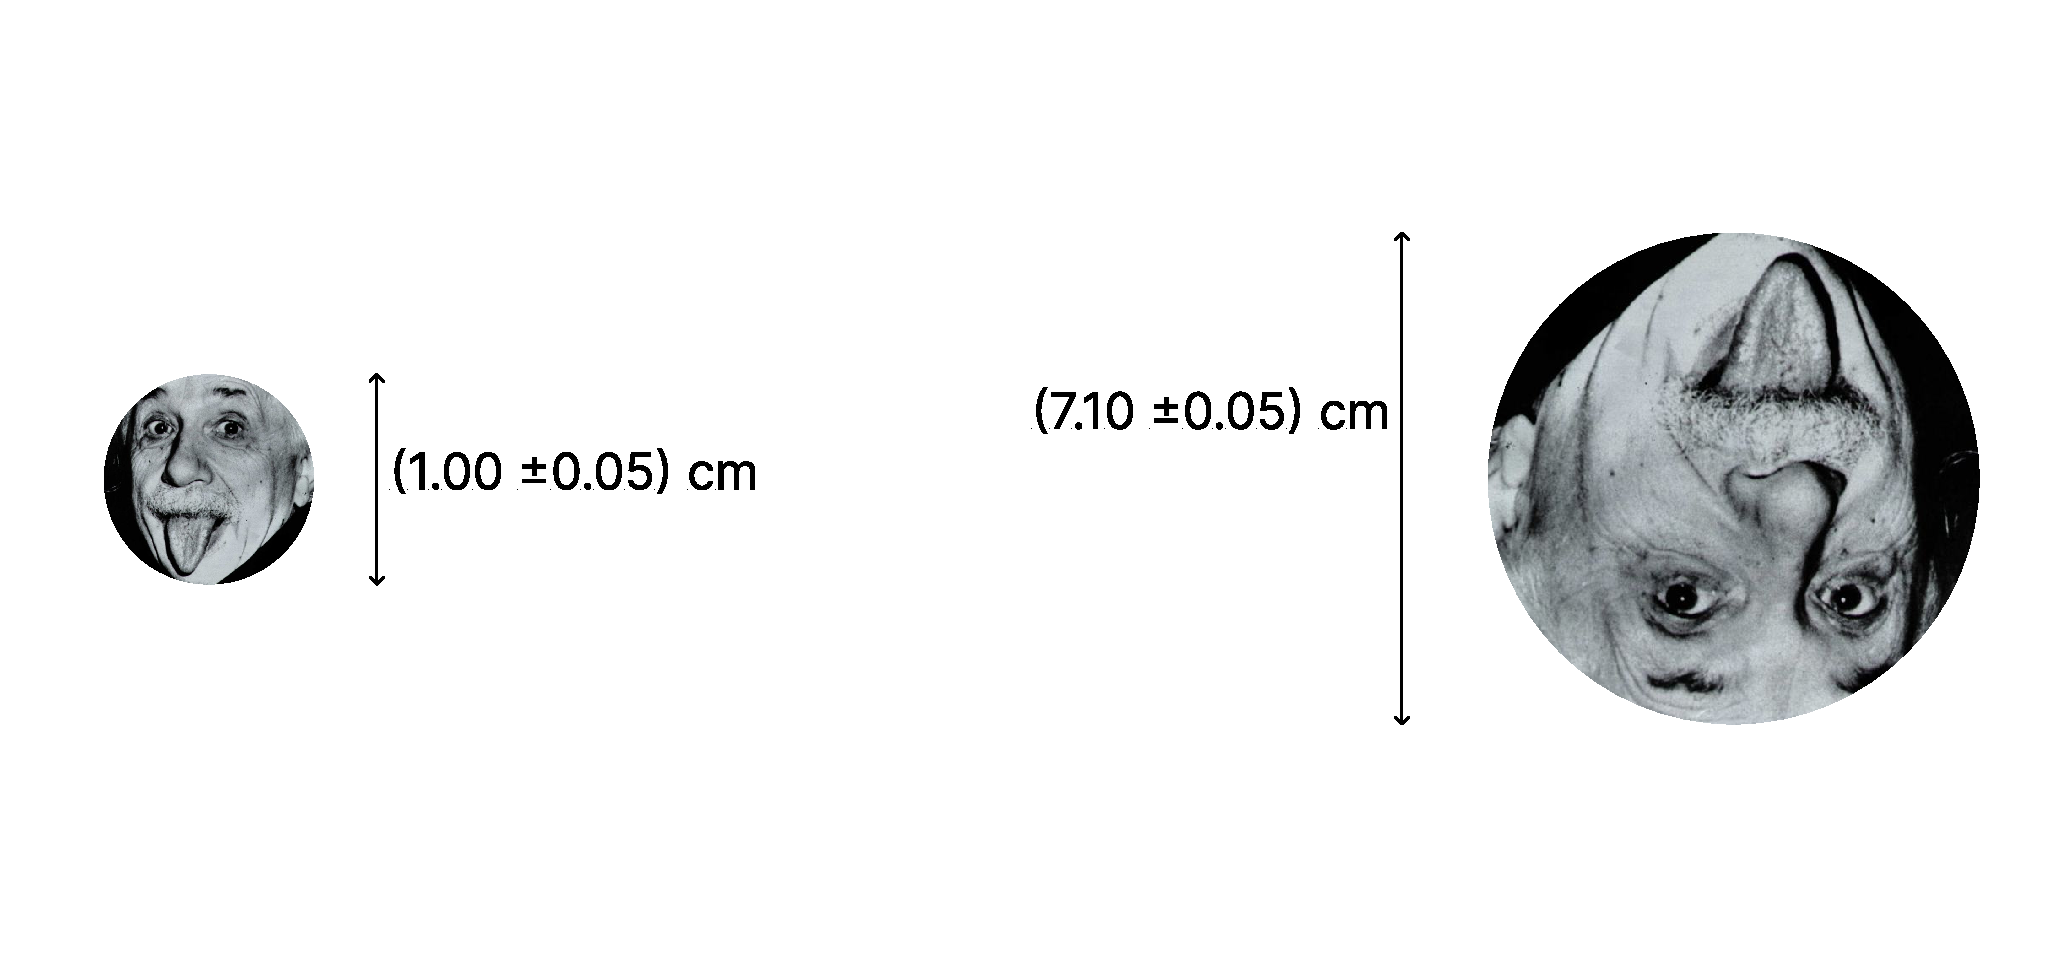
\includegraphics[width=0.7\pagewidth]{images/grandi.pdf}
        };
    \end{tikzpicture}
    \begin{tikzpicture}[remember picture,overlay]
        \node [anchor=south west] at (current page.south west) {%
            \tiny \color{black}\textbf{@HE-Arc, Laboratoire de physique}
        };
    \end{tikzpicture}
\end{frame}

\begin{frame}
    \begin{tikzpicture}[remember picture,overlay]
        \node [anchor=south east] at (current page.south east) {%
            
\includegraphics[scale=0.2]{images/lab_elements.png}
        };
    \end{tikzpicture}
    \begin{tikzpicture}[remember picture,overlay]
        \node [anchor=north west] at ([xshift=1.4cm,yshift=-1cm]current page.north west) {%
            \begin{minipage}{0.5\textwidth}
                \Huge\textbf{Mesures :} \\
                \Large\textbf{Loi du grandissement}
            \end{minipage}
        };
    \end{tikzpicture}
    \begin{tikzpicture}[remember picture,overlay]
        \node [anchor=center] at (current page.center) {%
            \begin{minipage}{0.5\textwidth}
                \Large
                \begin{empheq}[box={\mymath}]{equation*}
                    m_y = (-7.1 \pm 0.4)
                \end{empheq}
                \begin{empheq}[box={\mymath}]{equation*}
                    m_{pq} = (-7.1 \pm 0.1)
                \end{empheq}
            \end{minipage}
        };
    \end{tikzpicture}
    \begin{tikzpicture}[remember picture,overlay]
        \node [anchor=south west] at (current page.south west) {%
            \tiny \color{black}\textbf{@HE-Arc, Laboratoire de physique}
        };
    \end{tikzpicture}
\end{frame}

\begin{frame}
    \begin{tikzpicture}[remember picture,overlay]
        \node [anchor=north west] at ([xshift=1.4cm,yshift=-1cm]current page.north west) {%
            \color{black}\Huge\textbf{Conclusion}
        };
    \end{tikzpicture}
    \begin{tikzpicture}[remember picture,overlay]
        \node [anchor=west] at ([xshift=1.4cm]current page.west) {%
            \begin{minipage}{0.5\textwidth}
                \begin{itemize}
                    \item Les mesures sont en accord avec les lois
                    \item Les incertitudes sont faibles
                    \item Les buts de l'étude sont atteints
                \end{itemize}
            \end{minipage}
        };
    \end{tikzpicture}
    \begin{tikzpicture}[remember picture,overlay]
        \node [anchor=east] at ([xshift=-1.4cm]current page.east) {%
            \begin{minipage}{0.4\textwidth}
                \begin{empheq}[box={\mymath}]{equation*}
                    f_{calc} = (9.8 \pm 0.2) \textrm{cm}
                \end{empheq}
                \begin{empheq}[box={\mymath}]{equation*}
                    f_{fab} = (10 \pm 0.1) \textrm{cm}
                \end{empheq}
                \vspace{1cm}
                \begin{empheq}[box={\mymath}]{equation*}
                    m_y = (-7.1 \pm 0.4)
                \end{empheq}
                \begin{empheq}[box={\mymath}]{equation*}
                    m_{pq} = (-7.1 \pm 0.1)
                \end{empheq}
            \end{minipage}
        };
    \end{tikzpicture}
    \begin{tikzpicture}[remember picture,overlay]
        \node [anchor=south west] at (current page.south west) {%
            \tiny \color{black}\textbf{@HE-Arc, Laboratoire de physique}
        };
    \end{tikzpicture}
\end{frame}

\begin{frame}
    \begin{tikzpicture}[remember picture,overlay]
        \node [anchor=south east] at (current page.south east) {%
            
\includegraphics[scale=0.2]{images/lab_elements.png}
        };
    \end{tikzpicture}
    \begin{tikzpicture}[remember picture,overlay]
        \node [anchor=center] at (current page.center) {%
            \begin{minipage}{\textwidth}
                \centering
                \color{black}\Huge\textbf{Merci beaucoup} \\
                \color{black}\Large\textbf{Questions ?} \\
                \vspace{1cm}
            \end{minipage}
        };
    \end{tikzpicture}
    \begin{tikzpicture}[remember picture,overlay]
        \node [anchor=south west] at (current page.south west) {%
            
\includegraphics[scale=0.7]{images/logo_hearc_big.eps}
        };
    \end{tikzpicture}
\end{frame}

\end{document}
